\documentclass{beamer}
\usetheme{Boadilla}
\usepackage{polski}
\usepackage[utf8]{inputenc}
\title{BTS Maintenance System }
\subtitle{Wykorzystane technologie}
 \author{Michał Błach, Kacper Szewczyk}
%\institute{Slyboots \& Zawodnik Company}
\date{\today}
\setbeamercovered{transparent}
\begin{document}
\begin{frame}
\titlepage
\end{frame}
\begin{frame}
\tableofcontents
\end{frame}

\section{Aplikacja kliencka}

\subsection{Projektowanie aplikacji i problemy z tym związane}
\begin{frame}{Znana sytuacja ?}
     \begin{columns}[T] % contents are top vertically aligned
      \begin{column}[T]{8cm} % alternative top-align that's better for graphics
          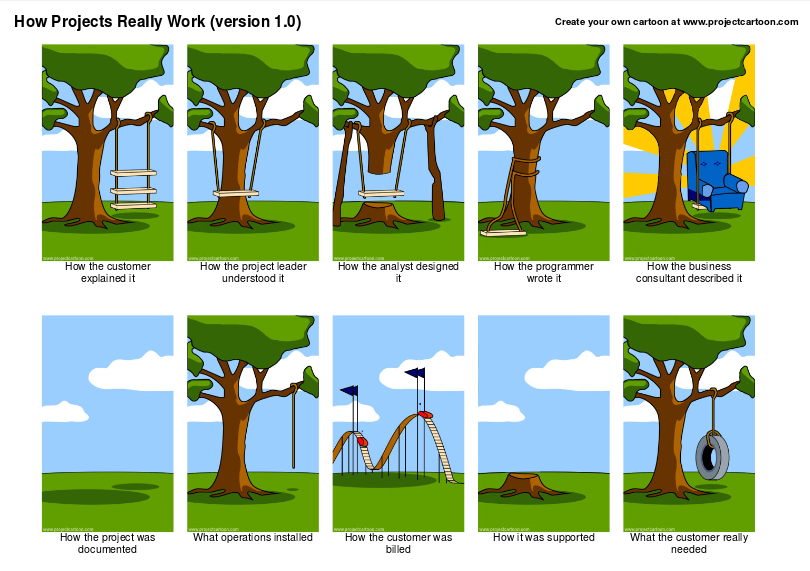
\includegraphics[width=8cm]{how_works.png}
     \end{column}
     \begin{column}[T]{4cm} % each column can also be its own environment
     \begin{block}<1->{Nowy projekt/zlecenie}
	Rozpoczynamy nowy projekt startup.\\
	Po długich rozmowach z potencjalnymi klientami udaje nam się skonkretyzować specyfikacje projektu.
	Rozpoczynamy implementacje, po czym okazuje się, że \dots 
\end{block}
     \end{column}
     \end{columns}
\end{frame}


\begin{frame}{Znana sytuacja ?}
     \begin{columns}[T] % contents are top vertically aligned
     
          \begin{column}[T]{7cm} % each column can also be its own environment
    % \begin{block}<1->{Nowy projekt/zlecenie}
   % \framesubtitle{<subtitle>}
	\begin{itemize}
    \item<1-> Firma zmieniła telefony służbowe pracowników
    \item<2-> Project Manager pracujący u klienta używa innego OS.
    \item<3-> Zaszla potrzeba użytkowania aplikacji na Notebook-u/Laptopie
    \item<4-> \dots
    \end{itemize}
%\end{block}
     \end{column}
      \begin{column}[T]{5cm} % alternative top-align that's better for graphics
          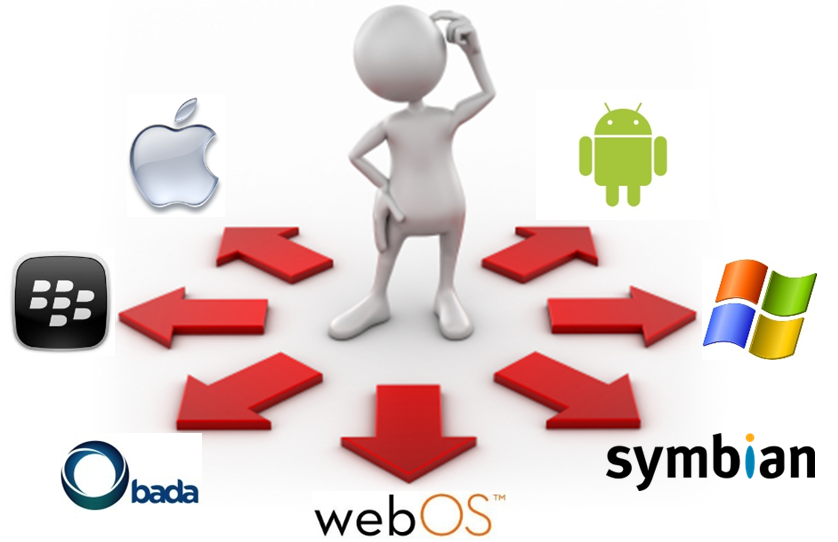
\includegraphics[width=5cm]{mobile.png}
     \end{column}
     \end{columns}
\end{frame}

\begin{frame}{Klasyczne rozwiązanie}
     \begin{columns}[T] % contents are top vertically aligned
      
     \begin{column}[T]{6cm} % each column can also be its own environment
     \begin{block}<1->{Zalety}
			\begin{itemize}
    \item<1-> Większa wydajność aplikacji
    \item<2-> Łatwy dostęp do interface-ów/urządzeń w urządzeniu, poprzez natywne odwołania
    \item<3-> \dots
    \end{itemize}
	\end{block}
     \end{column}
     \begin{column}[Tc]{6cm} % alternative top-align that's better for graphics
          
\includegraphics[width=6cm]{multi.jpg}
     \end{column}
     \end{columns}
\end{frame}


\begin{frame}{Klasyczne rozwiązanie}
     \begin{columns}[T] % contents are top vertically aligned
      
     \begin{column}[T]{6cm} % each column can also be its own environment
     \begin{block}<1->{Wady}
			\begin{itemize}
    \item<1-> Zatrudnienie wielu zespołów programistów do implementacji projeku na każdej 
    platformie.
    \item<2-> Powielanie tego samego kodu.
    \item<3-> Utrzymywanie wiele projektów, co wiąże sie z zatrudnieniem wielu
    ludzi, z powodów czasowych i technologicznych.
    \item<4-> Niejednolitość interface na każdej platformie.
    \item<5-> \dots
    \end{itemize}
	\end{block}
     \end{column}
     \begin{column}[Tc]{6cm} % alternative top-align that's better for graphics
          
\includegraphics[width=6cm]{busy.jpg}
     \end{column}
     \end{columns}
\end{frame}

\subsection{Dostępne frameworki}
\begin{frame}
\frametitle{Corona}
\begin{figure}
 
\includegraphics[width=12cm,valign=t]{corona.png}
 \end{figure}
 \begin{block}{Opis z oficjalnej strony }
Corona's extensive API library enables everything from animation to networking with just a few lines of code. Whether you're building games or business apps, you see changes instantly in the Corona Simulator and can iterate extremely quickly. Development is done in Lua, a lightning-fast and easy to learn scripting language. Couple Corona with Corona Editor and/or Composer GUI you'll achieve even faster workflow. 
 \end{block}
\end{frame}

\begin{frame}
\frametitle{QT}
\begin{figure}
 
\includegraphics[width=8cm,valign=t]{qt.png}
 \end{figure}
 \begin{block}{Opis z oficjalnej strony }
You can write and recycle Qt application and device UI code to run on all your target devices. You can take your applications everywhere: embedded, desktop and mobile platforms. Qt lets you future-proof your “things” by making them platform independent. Should you want diversity between platforms, like a responsive UI design for different screen sizes, this is simple to implement with Qt, as well.
 \end{block}
\end{frame}

\subsection{Cordova}

\begin{frame}
\frametitle{Cordova}
\begin{figure}
 
\includegraphics[width=10cm,valign=t]{cordova.png}
 \end{figure}
 \begin{block}{Opis z oficjalnej strony }

 \end{block}
\end{frame}
\subsubsection{HTML5}
\begin{frame}
\frametitle{Frame1}
\end{frame}
\subsubsection{CSS3}
\begin{frame}
\frametitle{Frame1}
\end{frame}
\subsubsection{Java Script}
\begin{frame}
\frametitle{Frame1}
\end{frame}
\section{Zewnętrzny serwer do synchronizacji danych}
\begin{frame}
\frametitle{Frame2}
\end{frame}
\section{Webowy klient do zarządania danymi na serwerze zewnętrznym}
\begin{frame}
\frametitle{Frame2}
\end{frame}
\begin{frame}
\frametitle{What Are Prime Numbers?}
\begin{definition}
A \alert{prime number} is a number that has exactly two divisors.
\end{definition}
\end{frame}

\begin{frame}
\frametitle{There Is No Largest Prime Number}
\framesubtitle{The proof uses \textit{reductio ad absurdum}.}
\begin{theorem}
There is no largest prime number.
\end{theorem}

\begin{proof}
\begin{enumerate}
\item<1-> Suppose $p$ were the largest prime number.
\item<2-> Let $q$ be the product of the first $p$ numbers.
\item<3-> Then $q + 1$ is not divisible by any of them.
\item<1-> But $q + 1$ is greater than $1$, thus divisible by some prime
number not in the first $p$ numbers.\qedhere
\end{enumerate}
\end{proof}
\uncover<4->{The proof used \textit{reductio ad absurdum}.}
\end{frame}

\end{document}



\end{document}
